\documentclass[a4paper]{article}
\usepackage{graphicx}
\usepackage{amsmath}
\usepackage[margin=1in]{geometry}
\usepackage{fancyhdr}

\pagestyle{fancy}
\fancyhead[l]{Afando Rafid F.A}
\fancyhead[c]{Classical Mechanics Homework 1}
\fancyhead[r]{November 22, 2023}

\newcommand*{\details}[2]{% <--- there was a spurious space here
  \textbf{#1} & : #2 \\
}

\begin{document}
\thispagestyle{plain}
\Large{\textbf{Classical Mechanics : Homework 1}}\\
\vskip 0.25cm
\begin{tabular}{l@{\hspace{2cm}}l}
    \details{Class}{B}
    \details{Instructor}{Ahmad Ataka Awwalur Rizqi}
    \details{Author}{Afando Rafid Falah As Shidiq}
    \details{NIM}{23/516817/TK/56823}
    \details{Date}{November 22, 2023}
\end{tabular}
\vskip 0.25cm
\hline\hline
\vskip 0.5cm
\Large{\textbf{Problem 1 : Rigid Body}}\\
\begin{center}
    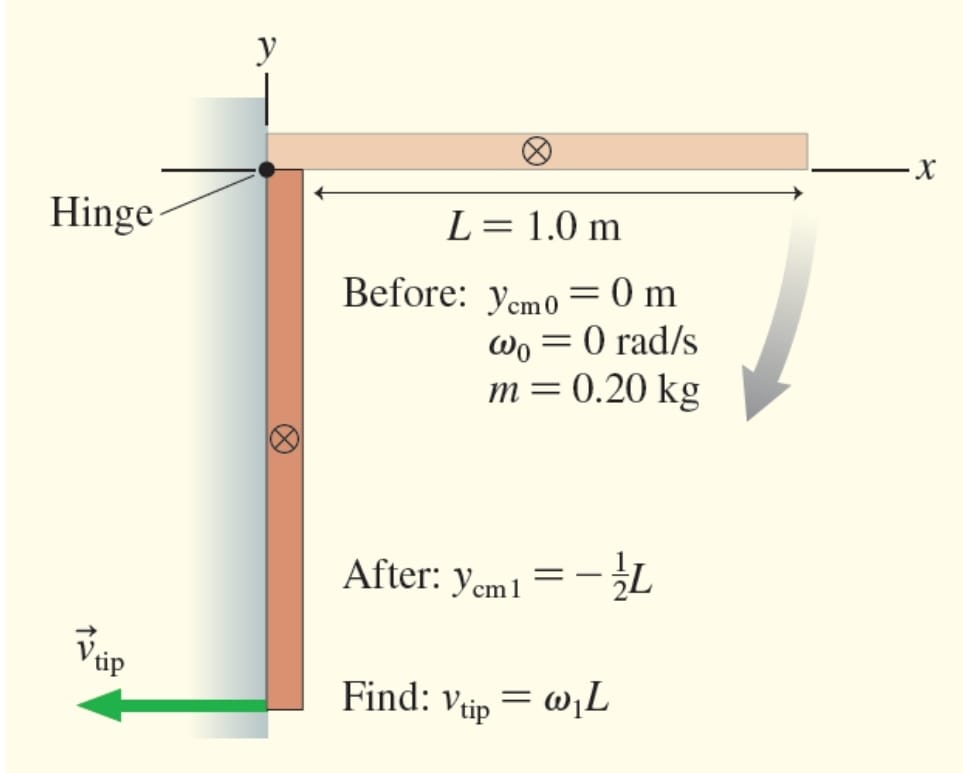
\includegraphics[width=7cm]{hinge.png}    
\end{center}
\large{\textbf{Question :}}\\
Find $v_{tip}=\omega_1L!$\vskip 0.5cm
\noindent \large{\textbf{Answer :}}\\
$$ME_i=ME_f$$
$$\frac{1}{2}I{\omega_i}^2+Mgy_i=\frac{1}{2}I{\omega_f}^2+Mgy_f$$
$$\frac{1}{2}I(0)+Mg(0)=\frac{1}{2}I{\omega_f}^2+Mgy_{cm1}$$
for a rod that rotates at the end ($I=\frac{1}{3}ML^2$)
$$0=\frac{1}{2}\left(\frac{1}{3}ML^2\right){\omega_f}^2+Mg\left(-\frac{1}{3}L\right)$$
$$0=\frac{1}{6}ML^2{\omega_f}^2-\frac{1}{2}MgL$$
$$\frac{1}{6}L{\omega_f}^2=\frac{1}{2}g$$
$${\omega_f}^2=\frac{3g}{L}$$
$$\omega_f=\sqrt{\frac{3g}{L}}$$

\newpage
$$v_{tip}=\omega_fL$$
$$v_{tip}=\sqrt{\frac{3g}{L}}L$$
$$v_{tip}=\sqrt{3gL}$$
$$v_{tip}=\sqrt{3(9.8)1}$$
$$v_{tip}=5,42$$
So, $v_{tip}$ at the end of the rod is $5,42$ m/s.

\end{document}
